% Szablon pracy inżynierskiej/magisterskiej 
% Autor: Wojciech Domski <wojciech.domski@pwr.edu.pl>
%
% Oryginalna wersja rozwijana przez dra inż. Adama Ratajczaka
% 
% Lista zmian:
% * 2024.01.05 Polecenie \zang oraz sekcja podział┐ pracy.
% * 2022.12.17 Dodano możliwość dodania streszczenia i słów 
%              kluczowych. Do tego czelu należy wykorzystać polecenie 
%              \summary
% * 2022.09.04 Dodatkowe uwagi o rysunkach i równaniach.
% * 2022.06.28 Dodanie uwag i wskazówek.
% * 2022.03.14 Zmiana kodu jednostki
% * 2022.03.14 Wykorzystanie nowej klasy mgr.cls dla W12N
% * Uproszczenie szablonu oraz uzupełnienie wymaganych 
% informacji

%Przykładowy plik ułatwiający złożenie projektu dyplomowego inżynierskiego.
%UWAGA: Generowany napis na stronie tytułowej o treści PROJEKT DYPLOMOWY INŻYNIERSKI został zaproponowany przeze mnie i nie jest, póki co, potwierdzony przez władze wydziału. Przed ostatecznym oddaniem tak złożonej pracy należy upewnić się jaka powinna być treść tego napisu. W momencie gdy uzyskam informację na temat treści tego napisu, dokonam niezbędnych zmian w źródłach.

\documentclass[eng,printmode]{mgr}
%opcje klasy dokumentu mgr.cls zostały opisane w dołączonej instrukcji

%poniżej deklaracje użycia pakietów, usunąć to co jest niepotrzebne
\usepackage{polski} %przydatne podczas składania dokumentów w j. polskim
%\usepackage[polish]{babel}%alternatywnie do pakietu polski, wybrać jeden z nich
\usepackage[utf8]{inputenc} %kodowanie znaków, zależne od systemu
\usepackage[T1]{fontenc} %poprawne składanie polskich czcionek

%pakiety do grafiki
\usepackage{graphicx}
\usepackage{subfigure}
\usepackage{psfrag}

%pakiety dodające dużo dodatkowych poleceń matematycznych
\usepackage{amsmath}
\usepackage{amsfonts}

%pakiety wspomagające i poprawiające składanie tabel
\usepackage{supertabular}
\usepackage{array}
\usepackage{tabularx}
\usepackage{hhline}

%różne pakiety
\usepackage{hyperref} % linki

%DODANE
\usepackage{float}
\usepackage{mathtools}
\usepackage[T1]{fontenc}

%pakiet wypisujący na marginesie etykiety równań i rysunków zdefiniowanych przez \label{}, chcąc wygenerować finalną wersję dokumentu wystarczy usunąć poniższą linię
%\usepackage{showlabels}

%definicje własnych poleceń
\newcommand{\R}{I\!\!R} %symbol liczb rzeczywistych, działa tylko w trybie matematycznym
\newtheorem{theorem}{Twierdzenie}[section] %nowe otoczenie do składania twierdzeń

%dane do złożenia strony tytułowej
\title{Wykorzystanie modelu generatywnego do rozszerzenia zbioru danych}
\engtitle{English title}
\author{Adam Jankowiak}
\supervisor{dr inż. Wojciech Domski}

%\date{2008} %standardowo u dołu strony tytułowej umieszczany jest bieżący rok, to polecenie pozwala wstawić dowolny rok

%poniżej jest lista kierunków i specjalności na wydziale elektroniki, należy wybrać właściwe lub dopisać jeśli nie ma odpowiednich
\field{Informatyka Stosowana (IST)}
\specialisation{Projektowanie Systemów Informatycznych}

%tutaj zaczyna się właściwa treść dokumentu
\begin{document}
\bibliographystyle{plabbrv} %tylko gdy używamy BibTeXa, ustawia polski styl bibliografii

\maketitle %polecenie generujące stronę tytułową
\dedication{6cm}{To jest przykładowa treść opcjonalnej dedykacji, należy ją zmienić lub usunąć w całości polecenie \texttt{$\backslash$dedication}}

\summary{Streszczenie pracy w języku polskim. Powinno zawierać 
około 10 zdań podsumowując pracę.}
{Streszczenie pracy w języku angielskim.
Powinno zawierać około 10 zdań podsumowując pracę.
\textbf{Proszę wykorzystać np. Google Translator.}}
{Słowa kluczowe w języku polskim. Tutaj pojawiają się 
jedynie słowa kluczowe oddzielone przecinkami bez kropki na końcu. 
Liczba słów kluczowych to co najmniej 3, a maksymalnie 8}
{Słowa kluczowe w języku angielskim}

\tableofcontents %spis treści


\chapter{Wstęp}


% Czym jest model sztucznej inteligencji - rys historyczny itd.
Sztuczna inteligencja to ogólny termin, który opisuje zestaw metod i algorytmów umożliwiający maszyną na samodziale uczenie się, dostosowywanie do zmieniających warunków oraz naśladowanie ludzkiej inteligencji. Początki badań nad sztuczną inteligencją sięgają lat 50 XX wieku. Bardzo istotne dla rozwoju tej dziedziny było letnie seminarium naukowe Dartmouth workshop, podczas którego naukowcy dyskutowali na temat sztucznej inteligencji \cite{Dartmount}. To wydarzenie jest obecnie uważane za kamień milowy, który zapoczątkował pierwsze etapy prac nad tą nową technologią. 

% Jakie są problemy z nauczaniem takiego modelu - potrzebuje dużooo dancyh
Algorytmy uczenia maszynowego są powszechnie wykorzystywane do przetwarzania dużych ilości danych, wykrywania wzorców oraz podejmowania decyzji na podstawie zgromadzonej wiedzy. Systemy sztucznej inteligencji cechują się wysoką dokładnością oraz szybkością działania. Jedyną z głównych wad SI jest potrzeba wykorzystania odpowiednio dużego zbioru danych do skutecznego treningu modeli. W przypadku algorytmów do przetwarzania obrazów lub analizy języka naturalnego należy dostarczyć duże zbiory danych do wyuczenia sieci. Dodatkowo brak reprezentatywności próbek może doprowadzić do problemu związanego z jakością.   


% Rozszerzenie zbioru danych

% Czym jest model generatywny 
Generatywne sieci przeciwstawne (z ang. generative adversarial networks) znacząco wyróżniają się na tle innych metod sztucznej inteligencji. Nie tylko wykorzystują nowatorskie podejście do generowania danych, ale także dają możliwość tworzenia realistycznych fotografii. Generatywne sieci przeciwstawne po raz pierwszy zostały zaprezentowane w pracy autorstwa Iana Goodfellowa z 2014 roku \cite{goodfellow2014generative}. Cechują się one możliwością replikowania zbioru danych poprzez generowanie próbek. Model GAN składa się z dwóch powiązanych ze sobą sieci, generatora i dyskryminatora. Pierwsza z nich, odpowiada za generowanie nowych danych, natomiast druga dokonuje oceny wytworzonych próbek. W trakcie nauczania modelu, generator próbuje wytworzyć na tyle dobre próbki, żeby dyskryminator nie był w stanie odróżnić ich od prawdziwych danych. W trakcie treningu oba modele na wzajem rywalizują, dzięki czemu precyzja rośnie.      

Wśród modeli generatywnych można także wyróżnić głęboką konwolucyjną sieć generatywno adwersaryjną (z ang. deep convolutional generative adversarial network, DCGAN). Wykorzystuje ona warstwy konwolucyjne, dzięki czemu jest w stanie generować realistyczne zdjęcia wysokiej jakości.  

% Opisz model, sieć która będzie wykorzystywana w porówaniu


% Napisz coś o nowych przepisach EU
Wraz z dynamicznym rozwojem SI, Unia Europejska zdecydowała się na wprowadzenie nowych przepisów mających na celu uregulować prawnie wykorzystanie algorytmach uczenia maszynowego w celu ochrony praw człowieka \cite{AI_Act}. Europejska ustawa o sztucznej inteligencji (z ang. \textit{EU Artificial Intelligence Act}) dzieli sztuczną inteligencję ze względu na zagrożenie jakie może wywierać na społeczeństwo. Pierwszą grupą są systemy niedopuszczalnego ryzyka, do których można zaliczyć klasyfikację punktową obywateli oraz kategoryzację ludzi. Przykładem jest system stosowany w chinach do klasyfikacji i oceniania społeczeństwa na podstawie dokonywanych płatności, zachowań w sieci oraz lojalności do rządu. Drugą grupą są systemy wysokiego ryzyka, które mają negatywny wpływ na bezpieczeństwo oraz prawa podstawowe obywateli. Dodatkowo wszystkie systemy będą musiały zostać zarejestrowane w bazie danych Unii Europejskiej.  

%DOKONCZ
%TUTAJ
%Trzecią grupą 






%Cele pracy
Celem pracy było sprawdzenie wpływu sztucznie wygenerowanych próbek na jakość modelu sieci neuronowej. W celu zrealizowania tego zadania, wykorzystana został sieć generatywna adwersarialna (z ang. generative adversarial networks, GAN), która jest w stanie wygenerować nowe, fikcyjne zdjęcia. Aby móc porównać wpływ sztucznie wytworzonych fotografii wykorzystany został model sztucznej inteligencji, który określa podobieństwo pomiędzy dwoma twarzami. W pracy porównano jakość dwóch modeli. Zbiór danych, wykorzystany do nauki pierwszej sieci, posiadał jedynie rzeczywiste zdjęcia, natomiast zbiór danych dla drugiego modelu zawierał także nowo wygenerowane obrazy. 






\section{Teza}

Możliwe jest zwiększenie dokładności modelu sztucznej inteligencji poprzez wykorzystanie technik generatywnych do stworzenia zbioru uczącego.  


\section{Podział pracy}

W rozdziale drugim zamieszczono opis działania generatywnych sieci przeciwstawnych. Rozdział czwarty zawiera opis przetwarzania danych oraz sposób trenowania modeli GAN. 


%TUTAJ
%TODO
%DOKONCZ

%W tej sekcji należy opisać co znajduje się w każdym z rozdziałów. Jedno, dwa zdania na rozdział. Piszemy w czasie przeszłym. Przykładowo W rozdziale drugim zamieszczono założenia projektowe dotyczące elektronicznej części projektu. Kolejny rozdział opisuje . . .. Rozdział czwarty zawiera informacje na temat przeprowadzonych badań symulacyjnych.








\chapter{Generatywne sieci przeciwstawne}

Generatywne sieci przeciwstawne należą do klasy modeli sztucznej inteligencji, które zrewolucjonizowały podejście do generowania danych syntetycznych. Algorytm został zaprezentowany w 2014 roku przez Iana Goodfellowa oraz jego współpracowników. GAN możne być wykorzystany do generowania fikcyjnych obrazów, dźwięków, tekstów czy nawet sekwencji wideo, za pomocą dostarczonych wzorców. 
Model składa się z dwóch niezależnych sieci neuronowych, które wzajemnie się trenują. Pierwsza z nich, zwana generatorem, odpowiada za tworzenie fikcyjnych próbek. Druga, dyskryminator, określa czy stworzone próbki są zbliżone do danych uczących. Na poniższym rysunku \ref{fig:GAN_rep}, przedstawiona została graficzna reprezentacja sieci GAN.

\begin{figure}[H]
	\centering
	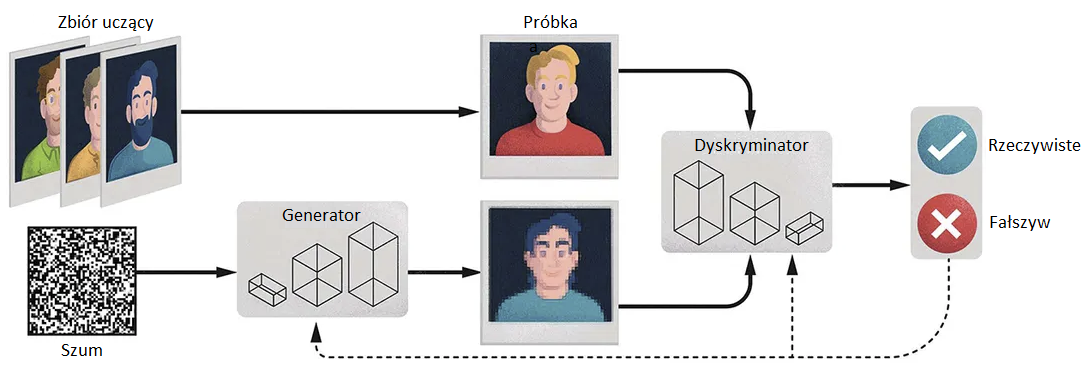
\includegraphics[width=0.8\textwidth]{figures/GAN_reprezentacja_graficzna.png}
	\caption{Graficzna reprezentacja sieci GAN.}
	\label{fig:GAN_rep}
\end{figure}

\section{Generator}

Generator jest siecią neuronową zdolną do tworzenia obrazów, dźwięków lub innych danych za pomocą dostarczonych wzorców. Proces uczenia polega na tworzeniu coraz to dokładniejszych próbek, które są następnie oceniane przez dyskryminator. Na początku treningu generator otrzymuje losowy wektor, który następnie, za pomocą rozkładu Gaussa, zostaje przekształcony w wygenerowany obraz. Podczas treningu generator stara się oszukać dyskryminator, tworząc próbki, które są coraz bardziej zbliżone do prawdziwych danych. Poprawa jakości generowanych obrazów odbywa się poprzez minimalizację funkcji straty, która mierzy, jak dobrze generator oszukuje dyskryminator. Głównym celem generatora jest wytworzenie sztucznych próbek, które są na tyle realistyczne, że dyskryminator nie jest w stanie określić czy dana próbka jest fałszywa. 






\section{Dyskryminator}

Dyskryminator to model sztucznej inteligencji, którego rolą jest określenie, czy wygenerowana próbka jest prawdziwa lub fałszywa. Danymi wejściowymi dla algorytmu są  zarówno prawdziwe próbki z zbioru danych jak i próbki wygenerowane przez generator.  Jako wyjście, dyskryminator zwraca wartość od 0 do 1, która określa prawdopodobieństwo, że ocenione dane są rzeczywiste. Wartość 1 określa, że dane wejściowe są prawdziwe, natomiast 0 wskazuje na fałszywe próbki. Dyskryminator jest trenowany tak, aby maksymalizować swoje umiejętności rozróżniania między prawdziwymi a fałszywymi danymi. Proces ten jest kluczowy, ponieważ determinuje on, jak dobrze generator potrafi tworzyć realistyczne próbki.



\section{Trening sieci}


Trening sieci GAN polega na iteracyjnym procesie współzawodnictwa pomiędzy generatorem a dyskryminatorem. Na każdym kroku treningu, generator tworzy nowe próbki, które są następnie oceniane przez dyskryminator. Dyskryminator stara się poprawić swoje umiejętności w wykrywaniu fałszywych danych, podczas gdy generator dąży do tworzenia coraz bardziej przekonujących próbek. Dyskryminator jest trenowany na dwóch zestawach danych: prawdziwych i fałszywych, wygenerowanych przez generator. Celem jest maksymalizacja funkcji straty dla próbek prawdziwych i minimalizacja dla próbek fałszywych. Generator jest trenowany na podstawie informacji zwrotnej od dyskryminatora. Generator stara się minimalizować funkcję straty dyskryminatora, która informuje, jak dobrze dyskryminator rozróżnia między prawdziwymi a fałszywymi próbkami. Proces ten kontynuuje się do momentu, gdy generator jest w stanie tworzyć próbki tak realistyczne, że dyskryminator nie może ich odróżnić od prawdziwych danych.


\section{Ocena sieci}


Głównym celem generatywnej sieci przeciwstawnej jest stworzenie na tyle precyzyjnego modelu generatora,  który będzie w stanie oszukać dyskryminator na tyle skutecznie, że generowane próbki będą nieodróżnialne od prawdziwych danych dla minimum połowy przypadków. W trakcie nauki model dyskryminatora i generatora uzyskuje coraz to większą dokładność dzięki czemu generowane próbki stają się coraz to lepsze. Ocena jakości generowanych danych może odbywać się na kilka sposobów. Pierwszym z nich jest przeglądanie wygenerowanych obrazów i porównywanie nich z rzeczywistymi danymi. Jest to dosyć skuteczna metoda pod względem precyzji, jednak pochłania bardzo dużą ilość czasu i jest mało skuteczna dla dużych zbiorów danych.  Drugą metodą jest wykorzystanie różnych miar jakości, takich jak odległość początkowa Frechta (z ang. \textit{Frechet Inception Distance, FID}), czy też wskaźnik incepcji (z ang. \textit{Inception Score , IS}). Wymienione miary są w stanie kwalifikować różnice pomiędzy prawdziwymi a wygenerowanymi próbkami. Wykorzystanie metody opartej na miarach jakości dobrze sprawdza się przy ocenianiu jakości dużych zbiorów danych. 




% trening na rzeczywistych, testowanie na rzeczywistych
% .. fikcyjnych, i fikcyjnych itd. 





\chapter{Wykorzystane technologie}

\section{Metody rozszerzenia zbioru}

\section{Platformy programistyczne wykorzystujące generatywne sieci przeciwstawne}





\chapter{Generowanie fikcyjnych zdjęć}

W celu stworzenia modelu umożliwiającego wygenerowanie fikcyjnych zdjęć twarzy wykorzystany został model generatywny StyleGAN2. Umożliwia on wygenerowanie nowych zdjęć na podstawie dostarczonej wcześniej bazy danych. Model został wybrany ze względu na wysoką dokładność tworzonych zdjęć oraz krótki czas trenowania modelu. StyleGAN2 został stworzony przez naukowców z firmy NVIDIA i jest jednym z bardziej zaawansowanych modeli generatywnych wykorzystywanych do tworzenia realistycznych zdjęć. Daje on także możliwość wydobycia odpowiednich cech na wygenerowanych obrazach poprzez dodanie odpowiednich etykiet (z ang. \textit{labels}) do zbioru uczącego.   

\section{Wykorzystany zbiór zdjęć}

Spośród dostępnych zbiorów, wybrana została baza zdjęć twarzy osób ORL \cite{ORL}. Została ona udostępniona przez laboratorium badawcze Olivetti z Wielkiej Brytanii (z ang. \textit{Olivetti Research Laboratory}), od którego pochodzi jego nazwa. Katalog zawiera fotografie twarzy wykonane 40 różnym osobom, z których każda miała wykonane 10 różnych zdjęć. Na załączonym rysunku \ref{fig:baza} można zobaczyć, że zdjęcia zostały zrobione w różnych chwilach, przy zróżnicowanym oświetleniu. Przedstawiają one różne wyrazy twarzy, a niektórzy ludzie mają nałożone lub zdjęte okulary. Dodatkowo wszystkie zdjęcia zostały wykonane na jednolitym czarnym tle, postacie są wyprostowane, ustawione frontalnie z dozwolonym minimalnym obrotem.  Obrazy są zapisane w formacie ośmiobitowym w skali szarości i mają rozmiar 112 na 92 piksele. 

 \begin{figure}[H]
	\centering
	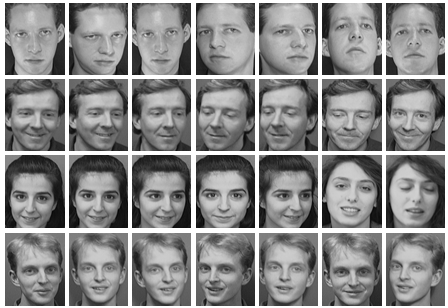
\includegraphics[width=0.5\textwidth]{figures/ORL_dataset.png}
	\caption{Przykładowe fotografie z bazy ORL.}
	\label{fig:baza}
\end{figure}



\section{Zmiana formatu zdjęć}

W celu ujednolicenia bazy wykonano konwersję formatu zdjęć. Przykład oryginalnego zdjęcia przed modyfikacjami znajduje się po lewej stronie rysunku \ref{fig:konwersja}. Fotografie zostały edytowane poprzez usunięcie górnych i dolnych wierszy zdjęcia. W wyniku tej operacji uzyskano próbki w formacie 92 na 92 piksele, co zostało przedstawione na środku rysunku \ref{fig:konwersja}. Wykorzystanie obrazów o proporcjach kwadratu było podyktowane możliwością uchwycenia nieregularności ludzkiej twarzy. Ostatni etap formatowania zdjęć polegał na przeskalowaniu zbioru do rozmiaru 64 na 64 piksele, co zostało przedstawione po prawej stronie rysunku \ref{fig:konwersja}. Zdjęcia o takich wymiarach zawierają wystarczającą ilość informacji potrzebnych do wytrenowania sieci GAN. 

 \begin{figure}[H]
	\centering
	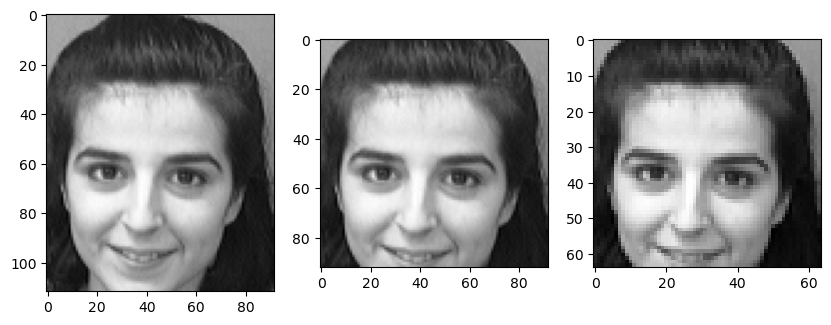
\includegraphics[width=0.8\textwidth]{figures/konwersja.png}
	\caption{Zawiera fotografie o rozmiarze 112x92, 92x92 oraz 64x64 piksele.}
	\label{fig:konwersja}
\end{figure}



\section{Rozszerzenie zbioru}

Baza ORL zawiera 400 zdjęć twarzy, co uniemożliwia wyuczenie sieci i uzyskanie wysokiej precyzji. Aby zwiększyć liczbę przykładów, zastosowano rozszerzenie zbioru poprzez obracanie i zaszumianie zdjęć. Dodatkowo fotografie zostały obrócone o kąty 2$^{\circ}$, 4$^{\circ}$ i 6$^{\circ}$ w obu kierunkach, co ilustruje \ref{fig:obrot}, przez co liczba obrazów przedstawiających jedną osobę wzrosła z 10 do 70. Nowo powstałe przykłady są traktowane przez sieć jako odmienne od oryginalnych. Dzieje się tak, ponieważ algorytm wczytuje zdjęcia wierszami, a wprowadzenie rotacji zmienia układ pikseli w macierzy, co pozwala uzyskać większą liczbę danych.



\begin{figure}[H]
	\centering
	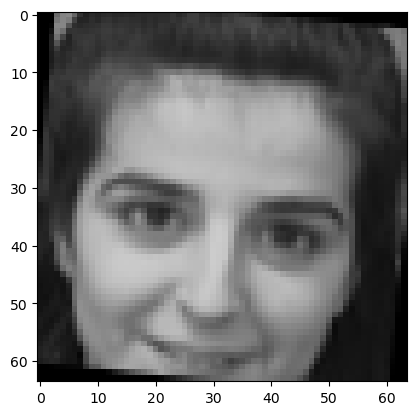
\includegraphics[width=0.38\textwidth]{figures/Obrot_6.png}
	\caption{Zdjęcie po dodaniu rotacji o kąt 6$^{\circ}$.}
	\label{fig:obrot}
\end{figure}


Drugą metodą zastosowaną w celu rozszerzenia zbioru było dodanie szumu. W tym celu do wszystkich zdjęć dodano szum Gaussa, co wpłynęło na wartości poszczególnych pikseli, rysunek \ref{fig:po_szumie}. Dzięki tej operacji liczba dostępnych próbek wzrosła z 70 do 140. Podobnie jak wcześniej, sieć neuronowa traktuje nowe przykłady jako różne od oryginałów.


\begin{figure}[H]
	\centering
	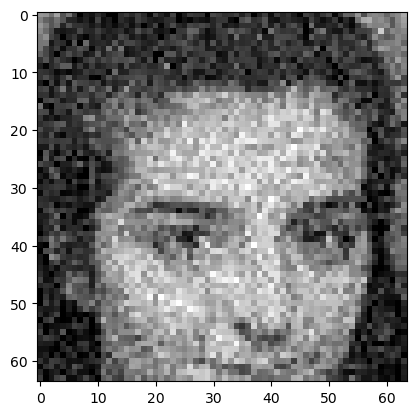
\includegraphics[width=0.38\textwidth]{figures/po_szumie.png}
	\caption{Zdjęcie po dodaniu szumu Gaussa.}
	\label{fig:po_szumie}
\end{figure}

Wykonanie rotacji oraz dodaniu zaszumienia do zdjęć, umożliwiło w łatwy i szybki sposób znacząco zwiększyć liczbę dostępnych fotografii. Po wykonaniu obu operacji uzyskano łącznie 5600 próbek.  





\section{Trenowanie modeli z wykorzystaniem StyleGan2}

Kolejnym krokiem generowania fikcyjnych zdjęć twarzy była nauka modelu GAN za pomocą wcześniej rozszerzonego zbioru rzeczywistych próbek. StyleGan2 daje możliwość dodania dodatkowej etykiety, która określa jakiego typu obraz ma zostać wygenerowany. W tym przepadku zdecydowano się na przebadaniu dwóch rodzai sieci. Pierwszy z nich zawierał jedynie zdjęcia tylko jednej osoby. Było to spowodowane możliwością mieszania się cudzych cech twarzy na jednym zdjęciu. Parametry wykorzystane podczas nauki sieci przedstawiono w tabeli \ref{tab:parametry_1}.

\begin{table}[H]
\centering
\small
\begin{tabular}{|l|l|}
\hline
Rozmiar partii          & 16     \\ \hline
Gamma                   & 3.2768 \\ \hline
Całkowity czas treningu & 100   \\ \hline
\end{tabular}
\caption{Przedstawia parametry wykorzystane do uczenia modelu stylegan2 bez etykiet.}
 \label{tab:parametry_1} 
\end{table}

gdzie:   

\begin{itemize}

\item Rozmiar partii (z ang. \textit{batch size}) oznacza liczbę próbek danych przetwarzanych jednocześnie podczas jednej iteracji treningowej.

\item Gamma (z ang. \textit{batch size}) określa, w jakim stopniu statystyki stylu są skalowane. Im większa wartość parametru gamma, tym bardziej intensywna jest zmiana stylu, podczas gdy mniejsza wartość gamma prowadzi do bardziej subtelnych zmian.

\item Całkowity czas treningu (z ang. \textit{total training duration}) oznacza całkowity czas treningu modelu, określany jest tysiącach iteracji. 

\end{itemize}





Głównymi wadami rozwiązania związanego z tworzeniem osobnego modelu dla każdej osoby jest znacznie dłuższy czas generowania modeli. Na poniższym rysunku \ref{fig:stylegan2_no_labels} przedstawione zostały rezultaty. Dla porównania po lewej stronie znajdują się rzeczywiste zdjęcia wybranej osoby, natomiast po prawej przedstawione zostały fikcyjne zdjęcia, wygenerowane przez model GAN. 


\begin{figure}[H]
	\centering
	\includegraphics[width=0.8\textwidth]{figures/stylegan2_no_labels.png}
	\caption{Porównanie rzeczywistych zdjęć z fikcyjnymi.}
	\label{fig:stylegan2_no_labels}
\end{figure}



Drugim sposobem generowania fikcyjnych zdjęć było wykorzystanie dodatkowych etykiet, które określały jaka osoba została przedstawiona na fotografii. W tym przypadku został stworzony tylko jeden model, który był w stanie generować zdjęcia różnych osób w zależności od podanej etykiety. Parametry wykorzystane podczas nauki sieci przedstawiono w tabeli \ref{tab:parametry_2}.

\begin{table}[H]
\centering
\small
\begin{tabular}{|l|l|}
\hline
Rozmiar partii          & 16     \\ \hline
Gamma                   & 3.2768 \\ \hline
Całkowity czas treningu & 1000   \\ \hline
Warunek                 & true   \\ \hline
\end{tabular}
\caption{Przedstawia parametry wykorzystane do uczenia modelu stylegan2 z etykietami.}
 \label{tab:parametry_2} 
\end{table}

\newpage

gdzie:   

\begin{itemize}

\item Warunek (z ang. \textit{conditional}) umożliwia generowanie obrazów na podstawie dodatkowych informacji wejściowych.

\end{itemize}

Zaletą podejścia związanego z wykorzystaniem dodatkowych etykiet jest znacząco zmniejszony czas nauki modelu. Na poniższym rysunku \ref{fig:stylegan2_labels} przedstawione zostało porównanie uzyskanych rezultatów z rzeczywistymi zdjęciami. Po lewej stronie pokazane zostały rzeczywiste zdjęcia, natomiast po prawej znajdują się fikcyjne fotografie, wygenerowane przez model StyleGan2 z dodatkowym wejściem określającym daną osobę.

\begin{figure}[H]
	\centering
	\includegraphics[width=0.8\textwidth]{figures/stylegan2_labels.png}
	\caption{Porównanie rzeczywistych zdjęć z fikcyjnymi.}
	\label{fig:stylegan2_labels}
\end{figure}

Jak można zauważyć na powyższych rysunkach \ref{fig:stylegan2_labels} oraz \ref{fig:stylegan2_no_labels}, wygenerowane zdjęcia są wysokiej jakości, zawierają także dużą ilość szczegółów, a co najważniejsze, wygenerowane zdjęcia osób są podobne do pierwowzorów. 







% dodaj zdjęcie z nauki, potrzeba udużo eopk


% Jak wygląda nauka? Jak podaje się parametry?

% Opisz jak przebierasz zdjęcia (określanie ostrości) 


\subsection{Odrzucanie błędnych próbek}

Wśród wygenerowanych fikcyjnych zdjęć twarzy można znaleźć także wiele różnych, niedoskonałych fotografii. Jak można zauważyć na poniższym rysunku \ref{fig:bledy}, model wygenerował zdjęcia, które posiadają różnego rodzaju niedoskonałości. Przykładowo zdjęcie w lewym górnym rogu przedstawia osobę z dwoma nosami, natomiast osoba w lewym górnym rogu ma zniekształcone oczy.

\begin{figure}[H]
	\centering
	\includegraphics[width=0.38\textwidth]{figures/Models_fault.png}
	\caption{Przedstawia błędnie wygenerowane próbki.}
	\label{fig:bledy}
\end{figure}

W celu wyeliminowania tych wad zdecydowano się wykorzystać dodatkowy model, który jest w stanie wykrywać twarze osób na zdjęciach. Zastosowanie tego modelu umożliwiło odrzucenie próbek, mna kórych znajdowały się mało wyraźne osoby. Dodatkowo wszystkie zdjęcia zostały przetworzone przez funkcje  Laplacian oraz Blure, które dostępne są w bibliotece Open CV. Laplacian wykorzystany był do wykrywania krawędzi w obrazie, dzięki czemu określono miarę ostrości obrazu. Blur wykorzystuje analizę częstotliwościowej obrazu, przy użyciu szybkiej transformaty Furiera (z ang. \textit{fast Fourier transform, FFT}), gdzie wyższa wartość wskaźnika rozmycia oznacza bardziej ostry obraz.


% Co robić, jak żyć?

% Model wykrywający twarz na zdjęciu
% Model określający ostrość, wybranie odpowiedniego progu






\chapter{Porównanie rezultatów}
% Wykorzystanie modelu z pracy inż

Decydując się zbadać, czy model GAN może rozszerzyć zbiór uczący, wykorzystano model oceniający podobieństwo między twarzami. Jako wejście algorytm przyjmuje zdjęcie, które przedstawia dwie twarze osób, natomiast jako wynik zwraca prawdopodobieństwo pomiędzy dwoma twarzami. Jako dane walidacyjne i dane treningowe zdecydowano się wykorzystać próbki rzeczywiste, żeby móc porównać ze sobą wszystkie stworzone modele.








% Opis tego modelu, jaka jest jego architektura, nawiązanie do pracy inż

% true - true
% fasle - true
%
%












\chapter{Podsumowanie}

%W podsumowaniu należy odnieść się do wyników jakie udało się uzyskać
%w trakcie pracy. Również tutaj jawnie należy się odnieść do tezy,
%pokazać w sposób logiczny, że cel w niej przedstawiony został osiągnięty.

%Zatem, podsumowanie powinno składać się z następujących części:
%\begin{enumerate}
%	\item 
%	Zdanie o wypełnieniu założeń pracy. 
%	\item
%	Następnie kilka lub kilkanaście zdań o projekcie co zostało wykonane. 
%	\item
%	Na końcu ewentualne dwa lub trzy problemy (maksymalnie), ta część powinna być 
%	dość krótka. Najlepiej podać propozycję rozwiązania.
%	\item
%	Koniec podsumowania powinien zawierać możliwe kierunki dalszego rozwoju. 
%	Jeżeli występowały w pracy problemy to proszę przedstawić owe problemy w 
%	trakcie pracy jako możliwe kierunki rozwoju, nie opisywać to jako problem 
%	i nie oznajmiać, że nie udało się czegoś wykonać.
%\end{enumerate}

\newpage
\addcontentsline{toc}{chapter}{Załącznik A}
\appendix
\thispagestyle{empty}

\chapter*{Załącznik A}
%\label{ch:ZalacznikA}

%W pracy, podczas której wytworzyliście Państwo oprogramowanie, modele,
%symulacje należy zawrzeć w pracy specjalny rozdział (dodatek), a
%w nim zawrzeć informację o dołączeniu do pracy płyty CD z odpowiednią
%adnotacją co do jej zawartości.

%W pracy powinien pojawić się załącznik znajdujący się po bibliografii 
%jako rozdział nienumerowany.

%Należy ogólnie opisać co znajduje się na dołączonej płycie CD. 
%Powinna to być lista (lub środowisko description).

%Np.

%Do pracy załączono płytę DVD zawierającą w~poszczególnych katalogach:

%\begin{description}
%\item
%\texttt{/Praca$\_$inzynierska.pdf} –- wersja cyfrowa pracy,
%\item
%\texttt{/Kod$\_$zrodlowy} –- kod źródłowy oprogramowania do ...,
%\item
%\texttt{/PCB.zip} -- projekt płytki PCB,
%\item
%\texttt{/Czesci$\_$mechaniczne.zip} -- archiwum z częściami mechanicznymi wykorzystanymi 
%w projekcie.

%\end{description}


\addcontentsline{toc}{chapter}{Bibilografia} %utworzenie w spisie treści pozycji Bibliografia
\bibliography{bibliografia} % wstawia bibliografię korzystając z pliku bibliografia.bib - dotyczy BibTeXa, jeżeli nie korzystamy z BibTeXa należy użyć otoczenia thebibliography

%opcjonalnie może się tu pojawić spis rysunków i tabel
% \listoffigures
% \listoftables
\end{document}

